\documentclass[12pt, a4paper]{article}
\usepackage[utf8]{inputenc}
\usepackage[spanish]{babel}
\usepackage{geometry}
\geometry{top=2.5cm, bottom=2.5cm, left=3cm, right=3cm}
\usepackage{graphicx}
\usepackage{tabularx}
\usepackage{array}

% Definición de un comando para las tablas/cajas de respuesta
\newcommand{\cajarespuesta}[2]{
    \vspace{0.4cm}
    \noindent \textbf{#1} \\
    \begin{tabularx}{\textwidth}{|X|}
    \hline
    #2 
    \vspace{0.2cm} \\ % Espacio para escribir el texto
    \hline
    \end{tabularx}
}

\setlength{\parindent}{0pt}

\begin{document}

% --- Portada ---
\begin{titlepage}
    \centering
    
\includegraphics[width=0.8\textwidth]{C:/Users/Gibio/Desktop/tesis/LOGO-USM-HORIZONTAL_RGB.png} \\[1cm]
    
    {\Large \textbf{UNIVERSIDAD TÉCNICA FEDERICO SANTA MARÍA}} \\[0.2cm]
    {\large DEPARTAMENTO DE ELECTRÓNICA} \\[2.5cm]

    {\Huge \textbf{Tarea Nro 1: Autoconocimiento y Liderazgo}} \\[1.5cm]

    \begin{flushleft}
    {\Large \textbf{Información del Estudiante:}} \\[0.5cm]
    \textbf{Nombre:} Gabriel José Ignacio Zapata Salazar \\
    \textbf{Email:} gabriel.zapatas@usm.cl \\
    \textbf{Carrera:} Ingeniería Civil Telemática \\
    \textbf{Desafío PMM:} PinPON, Modelo predictivo para mantenimiento en redes de acceso FTTH \\
    \textbf{Fecha de entrega:} 20 de Abril de 2026
    \end{flushleft}
    
    \vfill

    {\large
    Programa Memorias Multidisciplinarias (PMM) \\
    Módulo de Liderazgo \\
    Sede San Joaquín \\
    2026
    }
\end{titlepage}

\newpage

% --- Contenido del Documento ---

\noindent
\textbf{Liderazgo - Tarea \#1} \hfill San Joaquín, 20 de Abril de 2026 \\[0.5cm]

\cajarespuesta{1. ¿Quién soy yo fuera de la Universidad?}{
    Fuera de la universidad sigo siendo yo. Con mis valores, mi personalidad, mi humor, etc.
    Puesto que, al ir a la universidad no solo me desempeño como alumno, sino, como el entusiasta electrónico, amigo
    , jugador de pokémon, hijo (considerando que de todas maneras, mi familia igual estudió en esta instución, entonces también vine sin estar en la calidad de alumno), etc.
}

\cajarespuesta{2. ¿Qué importante evento (1) me ha cambiado la vida?}{
    Considero que cada persona que conozco y me permite involucrarme en un vínculo con ella es un evento que me cambia la vida.
    Sea en calidad de amigo, familiar o pareja.
}

\cajarespuesta{3. ¿Dónde/cómo te ves en 5 años más?}{
    Con un hogar propio en el que me reuna con mis seres queridos.
}

\cajarespuesta{4. ¿Qué haría si fuera 10 veces más valiente?}{
    Actualmente no me veo limitado por la valentía. No obstante, en su momento hubiera estudiado otra carrera si hubiera tenido la valentía que tengo. Que de todas formas, hubiera sido en esta misma instución
}

\vspace{0.4cm}
\noindent \textbf{5. Dibujo y descripción en una línea del tiempo (5 eventos importantes):} \\
\begin{center}
    % Asegúrate de que el archivo se llame lineatiempo.png o cambia el nombre aquí
    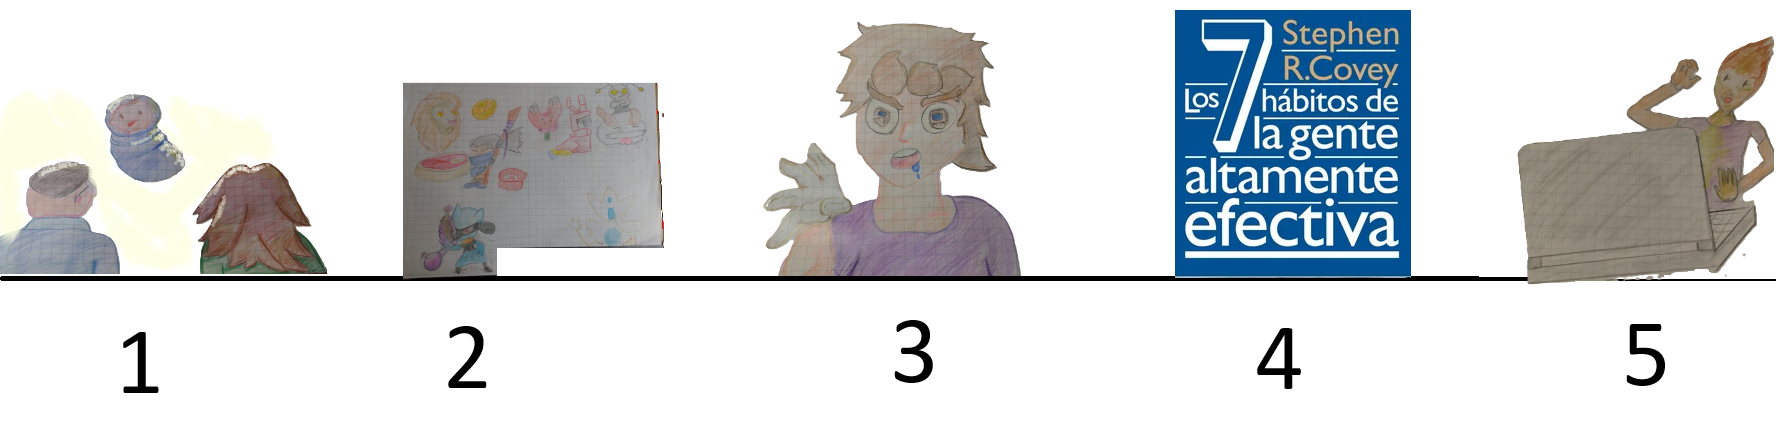
\includegraphics[width=\textwidth]{Linea temporal.png} 
\end{center}
\begin{tabularx}{\textwidth}{|X|}
    \hline
    Nacer 0 años. Parecera una nimiedad pero en donde y con quienes nací son indispensables en mi vida actual y como formé algunos de mis valores actuales.
    \\
Conocimiento de una computadora 3 años: Estableció mi curiosidad por todo lo tecnológico y los videojuegos\\

Establecer mis amistades 3-infinitos: Cada persona que hoy considero mi amigo son un grupo importante que le dedico mi tiempo y cariño todos los días.\\

Leer 7 hábitos para gente altamente efectiva 17 años: Este libro me animó a disfrutar leer de todo.\\

Descubrir la programación 20 años: Cuando di el ramo IWI131 descubrí una parte de la electrónica que me completo a aún mas y que se ha hecho uno de mis hobbies preferidos.
    \vspace{0.2cm} \\
    \hline
\end{tabularx}

\newpage

\cajarespuesta{6. ¿Consideras que tienes un buen conocimiento de ti misma/o? ¿Por qué?}{
    Considero que tengo un buen conocimiento de mi mismo. Esto debido a que tengo
    un núcleo de principios que me guían en mi vida diaria y que son acorde a mi objetivos de vida.
}

\cajarespuesta{7. ¿Qué es para mí el liderazgo? ¿Consideras que ejerces liderazgo en tu vida diaria?}{
      El liderazgo es poder conllevar voluntades en el sentido correcto, tanto de forma individual como grupal.
      Ejerzo liderazgo al momento de decidir que hacer en el día, a partir de mis objetivos ya planteados.
      También lo hago cuando con mis amigos decidimos que jugar. La forma en que lo hago es coordinando la palabra entre nosotros
      para maximizar nuestro tiempo juntos en lo que mas disfrutemos  todos.
}

\cajarespuesta{8. ¿Qué desafíos tengo/tenemos? (Selecciona uno y analiza su parte técnica y adaptativa)}{
    Con mi equipo tenemos el desafío de delimitar todos los puntos de falla en una fibra óptica.\\
    \textbf{Técnica:} Poder detectar los puntos de falla mas relevantes para el modelo para poder representar de manera fiable el sistema 
    \\
    \textbf{adaptativa:} Poder entender que aumenta o disminuye la satisfacción en los clientes de la fibra óptica.
}

\cajarespuesta{9. ¿Cómo voy a ejercer liderazgo en mi equipo de trabajo (PMM)?}{
    Con empatía, proyección y de forma íntegra. Entenderé las necesidades de mi compañero
    para sinergizar nuestro trabajo, escucharé de forma proactiva a mi profesor guía
    para desarrollar bien el proyecto y harémos planteamientos efectivos con mi supervisor.
    Considero que el liderazgo no solo se ejerce como líder, sino también, siendo un buen integrante de equipo para otro líder
}

\cajarespuesta{10. ¿Qué espero que pase en este curso de Liderazgo?}{
   Espero afilar la sierra en el ámbito de liderazgo.
   Considero que es una habilidad que tengo pero espero ver otro enfoque además de los que ya tengo y añadirlo
   a mi caja de herramientas de esta competencia.
}

\end{document}